%%=============================================================================
%% Proof of concept
%%=============================================================================
\graphicspath{ {./graphics/} }
\chapter{\IfLanguageName{dutch}{Proof Of Concept}{Proof Of Concept}}%

In dit hoofdstuk wordt de proof of concept uitgewerkt. De recent verkregen informatie wordt hierbij omgezet in de praktijk. De Proof Of Concept zal een beeld vormen van de oplossing voor het gestelde probleem. Als eerst zal er gekeken worden naar de gebruikte netwerkopstelling binnen Azure.
Vervolgens zal de gebruikte infrastructuur aan bod komen. Daarnaast zal er dieper worden ingegaan op Ansible en de bijhorende playbooks die zorgen voor de configuratie van de firewall. Verder wordt er gekeken naar de uitwerking van
het powershell script dan instaat voor het uitvoeren van controles op de ingevoerde data door de klant. Dit script zal alle zaken die hiervoor werden besproken samenbrengen tot 1 werkende geheel. 

\newpage

\section{Netwerkopstelling}
De netwerkopstelling die gebruikt wordt voor de Proof of Concept bestaat uit 2 virtuele machines elk in hun eigen subnet respectievelijk. In het eerste subnet met netwerkadres 172.22.2.0 bevindt zich een virtuele machine met het adres 172.22.2.5. Op deze machine staat een apache webserver geïnstalleerd. In het tweede subnet met netwerkadres 172.22.1.0 bevindt zich een virtuele machine met het adres 172.22.1.5. Deze machine zal dienen als host. Tussen deze twee subnets bevindt zich een firewall in de vorm van een Network Virtual Appliance (NVA) van Fortinet. Deze maakt gebruik van drie interfaces. Elk subnet is verbonden met één van deze interfaces. De derde interface is verbonden met de buitenwereld. Deze netwerkopstelling zorgt voor een ideale testomgeving. De mogelijkheid voorzien dat de host de webserver kan bereiken aan de hand van geautomatiseerde firewallrules met behulp van Ansible waarop, controle is uitgevoerd doormiddel van een powershell script, is het uitendelijke doel van deze Proof of Concept. In het werkveld zal deze opstelling complexer zijn dan wat hier wordt opgebouwd. Voor dit onderzoek is het voldoende om het simpel te houden. Dit is een perfecte manier om aan te tonen dat de onderzoeksvraag beantwoord wordt. 
\newline

\begin{tabularx}{0.8\textwidth} { 
  | >{\centering\arraybackslash}X 
  | >{\centering\arraybackslash}X 
  | >{\centering\arraybackslash}X
  | >{\centering\arraybackslash}X | }
 \hline
 Naam & Subnet & Adres & Firewall interface \\
 \hline
 Host  & 172.22.1.0  & 172.22.1.5 & 172.22.1.4 \\
\hline
 Webserver  & 172.22.2.0  & 172.22.2.5  & 172.22.2.4 \\
\hline
\end{tabularx}

\subsection{Topologie}

  % 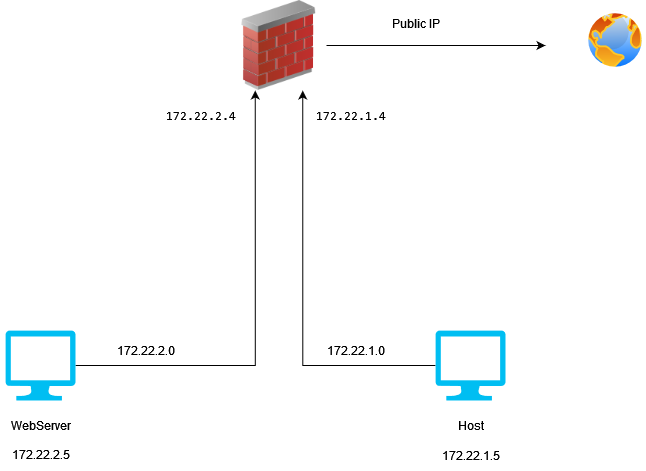
\includegraphics[width=100mm]{bachproef/graphics/topologie.drawio.png}
  % \label{fig:Topologie}

\section{Infrastructuur}
In dit onderdeel wordt besproken welke software , tools etc. gebruikt worden voor het opstellen van de Proof of Concept. Ook wordt er besproken wat er gebruikt wordt bij het uitwerken van de eerste versies en welke problemen dit met zich meebrengt om uiteindelijk niet voor die bepaalde optie te kiezen. Het is de bedoeling dat de infrastructuur snel en makkelijk opgezet kan worden door eender wie, zonder dat er veel extra software geïnstalleerd dient te worden.

Als eerste werd er gekeken naar een oplossing waarbij er manueel een linux virtuele machine werd opgezet. Hierop werd de nodige software (Ansible, ...) geïnstalleerd en al de benodigdheden geconfigureerd. Het werd al snel duidelijk dat dit een zeer omslachtige manier van werken was. Er was geen makkelijke manier om met een shared folder te werken. De enige manier om deze configuratie van de virtuele machine te delen was door het nemen van een image en deze te versturen. Deze bestanden kunnen groot zijn en zijn bijgevolg niet makkelijk te verdelen. Het was ook niet mogelijk om vanop afstand gemakkelijk de configuratie van de virtuele machine te gaan aanpassen. Hiervoor moest je steeds rechtstreeks inloggen op de machine en de juiste configuratie bestanden zoeken en aanpassen. Er was dus nood aan een vorm van automatisatie om zaken makkelijker te configureren. Het moest ook makkelijker door te geven zijn aan bijvoorbeeld een collega, zonder dat deze hiervoor een groot bestand moest binnenhalen. 
\subsection{Vagrant?}
Om de problemen op te lossen die kwamen kijken bij het manueel opstellen, werd er gebruik gemaakt van Vagrant. Dit is een handige tool voor de automatisatie en installatie van virtuele machines met een specifieke configuratie. Voor deze Proof of Concept werd er een virtuele machine opgezet met Vagrant waarop de Ansible software werd geïnstalleerd. Dit zorgde voor enkele problemen. 
\newline
\newline
Zo was het niet mogelijk voor de virtuele machine om een verbinding op te zetten met de firewall om hierop zaken te gaan uitvoeren met behulp van Ansible. Met Vagrant werken zou er bijgevolg ook tot leiden dat er allerlei zaken zouden moeten geïnstalleerd worden op de lokale host. Dit zorgt ervoor dat het niet zo vanzelfsprekend is om dit door te geven aan een collega. Hiervoor zou documentatie geschreven horen te worden om de werking van alles te begrijpen. Dit leidde tot de conclusie dat dit een te omslachtige manier van werken is , dit kon dus makkelijker. 
\newpage

\subsection{Docker!}
Aangezien Vagrant niet meteen gezien wordt als de beste oplossing, is er nood aan een alternatief. Wanneer er nood is aan een oplossing waarbij snel en efficiënt een instantie van een virtuele machine moet worden opgezet , waarbij flexibiliteit belangrijk is, blijkt Docker een goeie oplossing. De mogelijkheid om de configuratie op dockerhub te plaatsen zorgt voor een makkelijke distributie van de opstelling. Docker is bijgevolg de enige software die nodig is voor het opstellen en gebruiken van de gehele infrastructuur. Het installeren van deze software kan op twee manieren. In het geval van een Windows machines kan dit op twee verschillende manieren gebeuren. Dit kan enerzijds via de command line interface of anderzijds via een .exe bestand. Op Linux machines kan dit enkel via de command line interface. Hiervoor kan de documentatie van Docker geraadpleegd worden via \url{ https://www.docker.com/}. \newline

\subsubsection{DockerFile}
Docker maakt gebruik van een eigen bestandsformaat, namelijk een dockerfile. Deze dockerfile wordt gebruikt voor het configureren van instanties van een virtuele machine. Deze instanties worden images genoemd die later worden opgebouwd als in de vorm van een container. Deze containers bevatten enkel de software en functionaliteiten die meegegeven worden in de dockerfile. \newline

Hieronder worden enkele lijnen getoond afkomstig uit de dockerfile die gebruikt werd voor de opbouw van de Proof of Concept. 


\begin{lstlisting}
FROM ubuntu:22.04

RUN apt-get update && apt-get upgrade -y
RUN apt-get -y install python3 python3-nacl python3-pip libffi-dev vim
RUN ansible-galaxy collection install ansible.netcommon:4.1.0 

COPY ./credentials /root/.azure/
COPY ./azureProfile.json /root/.azure/
\end{lstlisting}
(code DockerFile, bijlage nr.2)

Het eerste wat meteen opvalt is de manier waarop het bestand is opgebouwd. Een Dockerfile is makkelijk leesbaar. Zo wordt er gebruik gemaakt van verschillende keywords. het keyword "FROM" (lijn 1) wordt gebruikt om te definiëren welke Operating system er gebruikt zal worden. In dit voorbeeld is de container een Linux machine die gebruik maakt van de Ubuntu versie 22.04 distributie. Verder wordt er gebruik gemaakt van het keyword "RUN" (lijn 3 en 4). Na dit keyword volgt er steeds een commando dat uitgevoerd dient te worden op de command line interface. In dit voorbeeld worden er verschillende packages , zoals python , pip , vim ,... geïnstalleerd bij het bouwen van de container. Het keyword "COPY" (lijn 6 en 7) wordt daarnaast gebruikt voor het kopiëren van bestanden, afkomstig van de lokale machine,naar de container. Lijn 4 zal zorgen voor een downgrade van de ansible.netcommon collectie. Dit is een collectie die helpt bij het automatiseren van netwerk management , security en cloud apparaten. Dit is dus een cruciale collectie voor deze Proof of Concept. De nieuwste versie van deze collectie zorgde weliswaar voor problemen bij het uitvoeren van de Ansible playbooks. Al snel werd duidelijk dat dit probleem veroorzaakt werd door de versie van de netcommon collectie. Later in hoofdstuk \ref{sec:Ansible} wordt hier dieper op in gegaan. 

\subsubsection{Docker compose}
Bij het opzetten van de gehele infrastructuur werd gebruik gemaakt van docker compose. Dit is een tool die helpt bij het definiëren en delen van omgevingen die bestaan uit meerdere containers. Wanneer aan de hand van een Dockerfile een container wordt aangemaakt wordt deze opgeslagen in een algemene file. Dit zorgt ervoor dat er een soort van bibliotheek van containers ontstaat. Met Docker compose is het bijgevolg mogelijk om één van de containers te kiezen om deze aan te maken en op te starten. Docker compose zorgt dus eigenlijk voor de initialisatie en bouw van de containers. Dit gebeurt aan de hand van de images die aangemaakt worden in de Dockerfile. Docker compose maakt gebruik van een file in YAML formaat. In deze file is het mogelijk om allerlei instellingen mee te geven die moeten worden uitgevoerd bij het opstarten van de Docker container. Hieronder wordt de file vertoond die gebruikt werd bij de opzet van de Proof of Concept. \newline

\begin{lstlisting}
version: "3.7"

services:
    fortigate-zero-touch:
        tty: true # Container restarts without
        container_name: ansible
        # Name of image you made with the Dockerfile
        image: ansible:key
        environment:
         - TZ=Europe/Brussels 
        # Creation of shared folders / files     
        volumes:
            - ../../projects:/projects
            - ../../output:/output
            - ./ansible.cfg:/etc/ansible/ansible.cfg
        # Directory in which container will start
        working_dir: /projects
        restart: unless-stopped
\end{lstlisting}

Zoals hierboven vermeld is het mogelijk om enkele instellingen mee te geven bij de opstart van de Docker container. Lijn 4 en 5 zorgen ervoor dat de container interactieve input van de gebruiker gaat accepteren. Docker is niet gemaakt om 24/7 containers te laten draaien. Docker dient enkel om achterliggend iets uit te voeren. Vanaf het moment dat er niets meer wordt uitgevoerd of draait op de container sluit deze automatisch af. Zijn taak zit er dan op. Voor deze use case is het echter wel nodig dat de docker container blijft draaien ookal wordt er niets meer uitgevoerd. Omwille hiervan wordt tty op true gezet. Op lijn 6 wordt er een naam gedefinieerd voor de container die zal aangemaakt worden. Lijn 8 geeft op zijn beurt aan welke image , die aangemaakt werd aan de hand van de Dockerfile, er gebruikt dient te worden.Lijn 10 wordt gebruikt voor het definiëren van de tijdszone waarin de container zich moet bevinden. Vervolgens zorgen lijn 12 tot en met 15 voor gedeelde mappen van de host naar de container. Dit zorgt ervoor dat het mogelijk is aanpassingen te maken op de container met behulp van Visual Studio Code. Dit werkt gemakkelijker dan rechtstreeks te werken op de container. Ten slotte zorgen de twee laatste lijnen ervoor dat de container zal initialiseren in de /projects directory.


\section{Oplossing!}
Tijdens dit onderdeel zal de gevonden oplossing voor het gegeven probleem aan bod komen. Er zal gedetailleerd ingegaan worden op de verschillende aspecten die nodig waren om de Proof of Concept tot een goed einde te brengen. Dit zal dan vooral gaan over de manier waarop Ansible gebruikt wordt en hoe dit te integreren met Powershell om controle uit te voeren op de input van de klant. 

\subsection{Ansible}
\label{sec:Ansible}
Dit onderdeel zal dieper ingaan op Ansible. Hieronder valt de werking van Ansible en de gebruikte playbooks. Deze playbooks liggen aan de basis van de oplossing voor het probleem. 

\subsubsection{Hoe?}
Ansible is zoals vermeld in \ref{sec:Wat is ansible}, een open source tool die het mogelijk maakt de configuratie van virtuele machines, zowel on premise als in de cloud, te automatiseren. Ansible maakt hiervoor gebruik van playbooks die in YAML formaat geschreven zijn. Hierin wordt de gewenste configuratie gedefinieerd. Deze configuratie wordt bijgevolg doorgestuurd naar de corresponderende machine die gedefinieerd dient te worden in deze YAML file.
\newline
\newline
\subsubsection{Inventory file}
Alle gekende machines die geconfigureerd horen te worden , moeten worden opgenomen in een inventory file. Deze inventory file bevat informatie die Ansible nodig heeft om een connectie vast te leggen met de gewenste machine. Zoals de naam van de machine en het ip adres. Daarnaast is er nog een extra vorm van authenticatie nodig. 

Hieronder de inventory file die gebruikt werd voor het opzetten van de Proof of Concept. 
\begin{lstlisting}
[fortigates]
fortigate1 ansible_host=192.168.2.2 External="port1" Internal="port2"
fortigate2 ansible_host=192.168.3.4 External="port1" Internal="port2"
[fortigates:vars]
ansible_network_os=fortinet.fortios.fortios
\end{lstlisting}


In een inventory file is het mogelijk om de verschillende machines te gaan groeperen. Op lijn één wordt de groep "fortigates" gedefinieerd waaronder twee machines vallen. Het is bijgevolg mogelijk om met ansible een groep aan te spreken en op deze manier alle machines in die groep dezelfde configuratie door te geven. Dit gebeurt op volgende manier :

\begin{lstlisting}
    ---
- hosts: "fortigates"
\end{lstlisting}

Daarnaast is het mogelijk om één enkele machine te configureren. Dit kan door gebruik te maken van de gekozen naam. Wanneer we de machine met ip 192.168.2.2 willen configureren ziet de start van de playbook er als volgt uit: 

\begin{lstlisting}
    ---
- hosts: "fortigate1"

\end{lstlisting}
Verder is het ook mogelijk om variabelen mee te geven, in de inventory file, die gebruikt kunnen worden door Ansible playbooks. Dit kunnen variabelen zijn die bij een specifieke machine horen. Zoals te zien op lijn één en twee van de inventory file. "External" en "Internal" zijn variabalen die de fysieke interfaces van de firewall gaan definiëren. De external interface is de interface verbonden met de buitenwereld (het internet). De interal interface is de interface verbonden met het netwerk, waar zich in deze Proof of Concept de host en de webserver zich bevinden. Deze variabelen zijn voor elke machine anders en moeten dus machine specifiek zijn. Voor variabele die globaal kunnen gebruikt worden door alles machines kan je een variabele lijst vasthangen aan een groep zoals te zien op lijn 4 van de inventory file. De variabele die hier worden gedefinieerd zijn globaal beschikbaar voor alle machines in de groep "fortigates". Dit vormt de basis, zonder deze informatie kan Ansible niet functioneren naar behoren. 
\newpage
\subsubsection{Authenticatie}
Zoals eerder besproken is er naast de naam en het ip adres van de machine nog een extra vorm van authenticatie nodig. Hiervoor zijn enkele mogelijkheden. Tijdens het opzetten van de Proof of Concept werden er verschillende methodes getest. 
\newline
\newline
Als eerste werd er gebruik gemaakt van gebruikersnaam en wachtwoord. Deze werden opgeslagen in de inventory file. 
Dat zag er als volgt uit: 

\begin{lstlisting}
    [fortigates]
fortigate01 ansible_host=192.168.2.2
ansible_user="User" ansible_password="Wachtwoord"

[fortigates:vars]
ansible_network_os=fortinet.fortios.fortios
\end{lstlisting}
Om gebruik te maken van gebruikersnaam en wachtwoord moeten er twee variabelen worden toegevoegd aan de inventory file namelijk "ansible\textunderscore user" en "ansible\textunderscore host" repectievelijk. Ansible zal automatisch gebruik maken van deze gegevens om zich te authenticeren. Dit is een makkelijke en snelle manier om ervoor te zorgen dat Ansible toegang krijgt tot de gewenste machine. Voor dit onderzoek daarentegen is dit geen bruikbare optie. De Ansible playbooks maken namelijk gebruik van een specifieke module voor het configureren van de firewall. Deze module maakt gebruik van API calls naar de firewall om de configuratie door te geven. Hiervoor is er nood aan een API access token. Gebruikersnaam en wachtwoord zijn voor de gewenste use case dus niet nuttig. Gebruikersnaam en wachtwoord zijn wel nuttig wanneer men enkele packages of applicaties wilt installeren met behulp van Ansible. Bijvoorbeeld voor het automatiseren van een SQL database. 
Daarnaast is het niet meteen een heel veilige manier van werken. Wanneer er gebruik gemaakt wordt van gebruikersnaam en wachtwoord zorgt dit voor een enorme kwetsbaarheid. Als men in handen komt van de inventory file , heeft deze persoon alle nodige info om de gehele machine over te nemen. Het is dus vanzelfsprekend dat dit geen goede methode is om te gaan gebruiken in een productie omgeving. Gebruik dit enkel met testen als doel.\newpage
De volgende methode die werd gebruikt zal wel zorgen voor een werkende oplossing. Zoals eerder vermeld maakt de module die gebruikt wordt voor de configuratie van de firewall gebruik van API calls. Hiervoor is bijgevolg een API access token nodig. Hiervoor moet er een API user aangemaakt worden met alle nodige rechten op de firewall. Het aanmaken van deze user genereerd vervolgens een API access token die gebruikt zal worden door Ansible voor de authenticatie die het uitvoeren van de API calls toelaat. Deze access token wordt vervolgens meegeven in de Ansible playbook als een variabele:
\begin{lstlisting}
    ---
- hosts: fortigates
  gather_facts: False
  connection: httpapi                                       
  collections:
   - fortinet.fortios
   - azure.azcollection
  vars:
    access_token: "token"
\end{lstlisting}
Op dit moment zijn enkel lijn 8 en 9 van belang, de andere zaken komen later tijdens dit onderdeel aan bod. Lijn 8 toont de manier om een lijst van variabelen, die gebruikt zullen worden in de playbook, te gaan definiëren. Op lijn 9 wordt de variabele access\textunderscore token gedeclareerd. Dit zal het bijgevolg mogelijk maken om deze playbook uit te voeren en de API calls door te sturen naar de firewall. Dit is dus een mogelijke manier van werken voor de use case van dit onderzoek. Net zoals dat het geval was bij het gebruik van gebruikersnaam en wachtwoord zou dit nooit in een productieomgeving mogen gebruikt worden. De access token staat als plain text in de Ansible playbook. Bijgevolg iedereen die de playbook in handen krijgt , kan configuratie doorvoeren op de firewall en op deze manier het gehele netwerk in handen nemen. Dit is dus geen veilige oplossing.
\newpage

bij vorige methodes was er een terugkerend probleem , namelijk de veiligheid. De informatie nodig voor het authenticeren is gemakkelijk te onderscheppen. Het moet dus mogelijk zijn om gebruik te maken van de access token zonder dat deze in plain text in een bestand terug te vinden is. De oplossing hiervoor is gebruik maken van een keyvault. Meer bepaald een Azure keyvault. Het is namelijk mogelijk om deze keyvault te gaan aanspreken doormiddel van API calls. Ook hiervoor is er een module aanwezig die geïnstalleerd kan worden op Ansible. De Azure keyvault gedraagt zich net zoals een klassieke password manager. 
%%=============================================================================
%% Methodologie
%%=============================================================================

\chapter{\IfLanguageName{dutch}{Methodologie}{Methodology}}%
\label{ch:methodologie}
Dit onderzoek zal in verschillende delen verlopen. In hoofdstuk twee werd er vooral informatie vergaard om het probleem zo goed mogelijk te begrijpen. Deze informatie werd verkregen aan de hand van een relevante literatuurstudie. Ook zal er beroep gedaan worden op interviews met belanghebbenden om op deze manier een requirements-analyse te kunnen uitvoeren. Dit zal ervoor zorgen dat er een optimale oplossing komt voor het beschreven probleem. De informatie wordt vervolgens gebruikt voor het opmaken van een Proof-of-Concept, waarin alle informatie zal toegepast worden in de praktijk. Dit Proof-of-Concept zal uiteindelijk ook het eindproduct zijn, waarin de oplossing van het probleem wordt weergegeven. Hierover zal ook een presentatie gegeven worden. Voor dit onderdeel wordt er beroep gedaan op communicatie met de copromoter en het bedrijf waarvoor dit onderzoek wordt uitgevoerd. Hiervoor zal een uitgebreide verzameling van software en hardware nodig zijn. Zo zal het mogelijk moeten zijn om gebruik te maken van alle Microsoft Azure features voor een zo'n specifiek mogelijke oplossing. Op deze manier kan er een realistisch scenario worden opgebouwd. Verder zal er ook eventueel beroep gedaan worden op een webapplicatie waarmee het mogelijk is firewall regels in te geven. Dit zal een zeer simpele applicatie zijn, geschreven in JavaScript. Deze applicatie is essentieel voor het oplossen van het gegeven probleem. Het is de bedoeling dat een klant aan de hand van een webapplicatie firewall regels kan doorsturen naar een firewall. Deze regels zullen worden opgenomen in een JSON-file. Op deze manier kan deze makkelijk worden geïmplementeerd in een script. Deze scripts worden gemaakt met Ansible in combinatie met een andere tool.  
Het zou kunnen dat tijdens het uitvoeren van het effectief onderzoek een betere oplossing wordt gevonden.
Concreet wordt er een Azure netwerk opgezet met een Network Virtual Appliance van het merk Fortigate. Op dit netwerk zal dan ook een webapplicatie draaien. Vervolgens worden er templates gebouwd, in verschillende Infrastructure as Code tools, voor het deployen van de gewenste firewall regels. Vervolgens zal er ook gekeken worden of deze manier van werken ook toegepast kan worden op een firewall van een andere vendor zoals Cisco. Voor dit onderdeel wordt ongeveer 40 uur geschat. Ten slotte worden de resultaten geanalyseerd en samen gebundeld in een concrete conclusie. 
%% TODO: Hoe ben je te werk gegaan? Verdeel je onderzoek in grote fasen, en
%% licht in elke fase toe welke stappen je gevolgd hebt. Verantwoord waarom je
%% op deze manier te werk gegaan bent. Je moet kunnen aantonen dat je de best
%% mogelijke manier toegepast hebt om een antwoord te vinden op de
%% onderzoeksvraag.



